% Part: sets-functions-relations
% Chapter: arithmetization
% Section:reals

\documentclass[../../../include/open-logic-section]{subfiles}

\begin{document}

\olfileid{sfr}{arith}{real}
\olsection{د حقيقي عددونو کرښه}

بل ګام دا ښودل دي چې له ناطقو عددونو څخه حقيقي عددونه څنګه
جوړېږي۔ تر هغې مخکښې بايد پوه شو چې د حقيقي عددونو
\emph{ځانګړتيا} څه ده۔

حقيقي عددونه ناطقو عددونو ته ډېر ورته چلند کوي۔ (په فني ډول، دواړه
د \emph{مرتبو ميدانونو} بېلګې دي؛ د دې د تعريف دپاره
\olref[check]{orderedfield} وګورئ۔) اوس که مو د
\olref[sfr][siz][]{chap} تمرينونه حل کړي وي، نو پوهېږئ چې حقيقي
عددونه له ناطقو عددونو په کلکه زيات دي؛ يعنې
$\cardless{\Rat}{\Real}$۔ دا خبره لومړے کانتور ثابته کړه۔ خو شاوخوا
دوه نيم زره کاله کېږي چې غير ناطق عددونه، يعنې هغه حقيقي عددونه چې
ناطق نۀ دي، پېژندل شوي دي۔ په رښتيا:
%\footnote{اوس: ``$\sqrt{2}$'' مثبت او منفي دواړو جذرونو ته يو شان اشاره کوي؛ خو په راتلونکو څو مخونو کښې به دا هېر کړم او يوازې مثبت جذر به په پام کښې نيسم۔}
\begin{thm}\ollabel{root2irrational}
$\sqrt{2}$ ناطق نۀ دے؛ يعنې $\sqrt{2} \notin \Rat$
\end{thm}

\begin{proof}
د تناقض دپاره فرض کړئ چې $\sqrt{2}$ ناطق دے۔ نو د ځينو طبيعي
عددونو $m$ او $n$ دپاره $\sqrt{2} = \nicefrac{m}{n}$۔ په حقيقت
کښې $m$ او $n$ داسې ټاکلے شو چې کسر نور نۀ شي ساده کېدے۔ په بيا
ترتيبولو $m^{2} = 2n^{2}$۔ له دې ځايه ثبوت په دوو لارو بشپړولے شو:

\emph{لومړے، په هندسي ډول} (د ټېننباوم په پيروۍ)۔\footnote{دا
ثبوت \cite{Conway2006} روايت کړے دے۔} دا مربعګانې په پام کښې ونيسئ:
\begin{center}	
	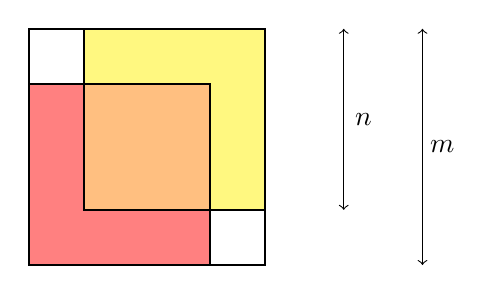
\begin{tikzpicture}
		\draw[thick] (0,0) rectangle (3,3);
		\draw[thick, fill=red!50] (0,0) rectangle (2.3,2.3);
		\draw[thick, fill=yellow!50] (0.7,0.7) rectangle (3, 3);
		\draw[thick, fill=orange!50] (0.7,0.7) rectangle (2.3, 2.3);
		\draw[<->] (4, 0.7)--(4, 3);
		\node at (4.25, 1.85) (n) {$n$};
		\draw[<->] (5, 0)--(5, 3);
		\node at (5.25, 1.5) (m) {$m$};
	\end{tikzpicture}
\end{center}
ځکه چې $m^2 = 2n^2$، هغه سيمه چې د ضلعې $n$ دواړه مربعګانې
يو پر بل راځي، له هغې سيمې سره مساوي مساحت لري چې له دغو دواړو
مربعګانو هېڅ يو نۀ ده پوښلې؛ يعنې د نارنجي مربع مساحت د دواړو
بې رنګه مربعګانو د مساحتونو له مجموعې سره مساوي دے۔ نو که د نارنجي
مربع ضلعه $p$ او د هر بې رنګه مربع ضلعه $q$ وي، نو $p^2 = 2q^2$۔
خو اوس $\sqrt{2} = \nicefrac{p}{q}$، چې $p < m$، $q < n$ او
$p, q \in \Nat$ دي۔ دا له دې خبرې سره تناقض لري چې $m$ او $n$
تر ټولو واړه ممکن عددونه ټاکل شوي وو۔
		
\emph{دويم، په صوري ډول۔} ځکه چې $m^{2} = 2n^{2}$، نو $m$ جفت
دے۔ (دا ښودل اسانه دي چې که $x$ طاق وي، نو $x^2$ هم طاق وي۔)
نو د کوم $r \in \Nat$ دپاره $m = 2r$۔ په بيا ترتيبولو
$2r^2 = n^2$،
		%				\begin{align*}
		%					(2q)^{2} &= 2n^{2}\\
		%					4q^{2} &= 2n^{2}\\
		%					2q^{2} &= n^{2}
		%				\end{align*}
نو $n$ هم جفت دے۔ په دې توګه $m$ او $n$ دواړه جفت دي، او له دې
امله کسر $\nicefrac{m}{n}$ نور \emph{ساده کېدے} شي۔ تناقض!
\end{proof}

په ضمن کښې دا انځوريز ثبوت موږ ته اجازه راکوي چې د \olref[his][set][mythology]{sec} مواد بيا وګورو۔ ټېننباوم (1927--2006) بشپړ معاصر رياضي پوه و؛ خو ثبوت بې شکه ښکلے، پوره دقيق او پر هندسي پوهېدنه ولاړ دے!

په هر حال، حقيقي عددونه تر ناطقو عددونو «ډېر پراخ» دي۔ په يوه معنا په ناطقو عددونو کښې «تشيالونه» شته چې حقيقي عددونه ئې ډکوي۔ وايرشټراس وپېژندله چې دا د حقيقي عددونو يو خاصيت بيانوي، کوم چې هغوے له ناطقو عددونو بېلوي؛ يعنې د بشپړتيا خاصيت: \emph{د حقيقي عددونو هر ناتش سټ چې پاسنی حد لري، تر ټولو لږ پاسنی حد هم لري۔}

دا ليدل اسانه دي چې ناطق عددونه د بشپړتيا خاصيت نۀ لري۔ د بېلګې په ډول له $\sqrt{2}$ څخه د وړو ناطقو عددونو دا سټ په پام کښې ونيسئ:
\[
	\Setabs{p \in \Rat}{p^2 < 2 \text{ يا }p < 0}
\]
دا په ناطقو عددونو کښې پاسنی حد لري؛ د بېلګې په ډول د دې ټول
!!{element}s له $3$ څخه واړه دي۔ \textbf{د ژباړې د نسخې سمون
(OLARI-002):} په انګرېزي سرچينه کښې د غړي له نښان وروسته يو بې
ځايه «کم تر» نښان پاتې و؛ دلته حذف شوے دے۔ خو د دې تر ټولو لږ
پاسنی حد څه دے؟ غواړو ووايو `$\sqrt{2}$'؛ خو همدا اوس مو وليدل
چې $\sqrt{2}$ \emph{ناطق نۀ} دے۔ او له $\sqrt{2}$ څخه لوے تر ټولو
لږ ناطق عدد نشته۔ نو دا سټ پاسنی حد لري خو تر ټولو لږ پاسنی حد نۀ
لري۔ له دې امله ناطق عددونه د بشپړتيا خاصيت نۀ لري۔

د دې پر خلاف، پيوستار «له معنوي پلوه بايد» د بشپړتيا خاصيت ولري۔ موږ يوازې دا نۀ غواړو چې $\sqrt{2}$ يو حقيقي عدد وي؛ غواړو د ناطقو عددونو د کرښې ټول «تشيالونه» ډک کړو۔ په رښتيا غواړو چې پخپله پيوستار هېڅ «تشيال» ونۀ لري۔ همدا هغه څه دي چې د بشپړتيا له لارې به ئې ترلاسه کړو۔

\end{document}
